\chapter{Design del Software} % Main chapter title

% \label{Chapter3} % For referencing the chapter elsewhere, use \ref{Chapter2} 
% Il primo modello del sistema che si è definito (\textit{modello di analisi}) è stato il risultato della prima fase, ovvero scaturito dalla fase di \textit{analisi e definizione dei requisiti}. \\
% \indent L’obiettivo di questo capitolo è invece descrivere il nuovo modello di sistema (\textit{modello di progettazione}), focalizzando l'attenzione prima sull'architettura scelta, poi sulla scomposizione del sistema in sottosistemi e infine sulla descrizione degli obiettivi di design raggiunti.

% \section{Modello architetturale client-server}

% Lo stile architetturale \textit{client-server} è stato organizzato in tre livelli (\textit{tier}) dove ognuno di  questi corrisponde a un nodo fisico di calcolo su cui è distribuito il sistema.

% \subsection{Livello di presentazione (\textit{client-tier})}
% Il livello di presentazione costituisce l'interfaccia utente (UI) del sistema e include la definizione dei layout visuali, delle schermate e della User Experience (UX) complessiva. Per lo sviluppo di questa applicazione desktop si è optato per l'impiego della libreria JavaFX.

% Questo layer assolve a due funzioni primarie:
% \begin{quote}
% \begin{enumerate}[label=\textit{\arabic*}]
%    \item (\textit{Visualizzazione dei dati}): eroga a schermo le informazioni precedentemente elaborate dal server.
  
%   \item (\textit{Acquisizione degli input}): intercetta le interazioni dell'utente (eventi di puntamento, digitazione di testo, selezioni da menu) e le inoltra ai livelli sottostanti. 
% \end{enumerate} 
% \end{quote}

% Il funzionamento si articola su un modello lineare: il livello riceve la richiesta dell'utente, la delega al layer della logica applicativa per la relativa elaborazione e, infine, renderizza il risultato ottenuto. \\
% \indent In linea con i principi di separazione delle responsabilità, questo livello non implementa alcuna logica decisionale: non valuta la validità o l'ammissibilità delle operazioni richieste, ma si limita a demandare tali verifiche al livello sottostante e a rappresentare graficamente l'esito della risposta ricevuta.

% \subsection{Livello della logica business (\textit{application-tier})}
% Il livello della logica applicativa rappresenta il modulo centrale del sistema: in esso risiedono i processi decisionali e l'esecuzione delle operazioni fondamentali per il funzionamento dell'applicazione.

% Per lo sviluppo di questo layer è stato impiegato il linguaggio Java unitamente al framework Spring.

% Questo layer comprende le seguenti funzionalità principali:
% \begin{quote}
% \begin{enumerate}[label=\textit{\arabic*}]
%    \item (\textit{Validazione dei dati e regole di dominio}): verifica la correttezza e la conformità delle informazioni in ingresso prima della loro elaborazione, applicando le business rules del dominio applicativo.
  
%   \item (\textit{Gestione della sicurezza}): controlla l'autenticazione degli utenti e ne definisce le autorizzazioni di accesso alle risorse.

%   \item (\textit{Integrazione di sistema}): coordina la comunicazione verso eventuali servizi o sistemi esterni.
% \end{enumerate} 
% \end{quote}

% Il layer risponde all'architettura sottostante esponendo le proprie funzionalità al livello di presentazione tramite API REST con scambio dati in formato JSON. Contestualmente, si interfaccia con il livello dei dati (Data Access Layer) per le operazioni di persistenza, lettura e aggiornamento delle informazioni.

% \subsection{Livello di gestione dei dati (\textit{database-tier})}
% Il livello di persistenza è responsabile della memorizzazione a lungo termine, del recupero e della salvaguardia della coerenza delle informazioni. Garantisce che i dati persistano inalterati anche a seguito della chiusura o del riavvio dell'applicazione. 

% Il layer comprende le seguenti funzionalità:
% \begin{quote}
% \begin{enumerate}[label=\textit{\arabic*}]
%    \item (\textit{Infrastruttura di memorizzazione}): si avvale di un database relazionale MySQL, strutturato mediante tabelle, vincoli di integrità e relazioni strutturali.
  
%   \item (\textit{Integrità dei dati}): assicura la correttezza e la coerenza del dominio informativo grazie all'impiego di vincoli strutturali (quali le chiavi esterne), che prevengono anomalie relazionali (ad esempio, l'esistenza di un'entità priva della propria associazione di riferimento).

%   \item (\textit{Principio isolamento}): l'accesso al database è consentito esclusivamente al livello della logica applicativa. Il layer di presentazione risulta totalmente disaccoppiato e non intrattiene alcuna comunicazione diretta con la base di dati.
% \end{enumerate} 
% \end{quote}

% \subsection{Perché conviene separare i livelli}
% I vantaggi di un'architettura a livelli sono:

% \begin{quote}
% \begin{enumerate}[label=\textit{\arabic*}]
%    \item (\textit{Manutenibilità}): Ogni componente ha una singola responsabilità. Trovare e correggere gli errori diventa più rapido e intuitivo.
  
%   \item (\textit{Flessibilità}): I moduli sono indipendenti. È possibile rinnovare l'interfaccia (es. da desktop a web) o cambiare il database senza impattare sul resto del sistema.

%   \item (\textit{Sicurezza}): Il database rimane isolato dagli accessi esterni diretti, mentre l'autenticazione e il controllo degli accessi sono gestiti in un unico punto sul server. 
  
%   \item (\textit{Scalabilità}): I livelli possono risiedere su server distinti, permettendo di potenziare solo le risorse realmente sollecitate.
% \end{enumerate} 
% \end{quote}

% \section{Decomposizione del sistema}
% Il sistema software in esame è stato progettato adottando un approccio modulare, partendo da componenti elementari più facilmente gestibili in fase di sviluppo e manutenzione. \\
% \indent In coerenza con l'architettura scelta, il sistema si articola in due macro-sottosistemi: \textit{Front-end} e \textit{Back-end}. Lo sviluppo del primo è stato affidato al team guidato da Giandomenico Iameo, mentre il secondo è stato coordinato dal team di Ubaldo Musto. \\
% Ciascun sottosistema è stato a sua volta suddiviso in moduli minori, seguendo il principio di separazione delle responsabilità. \\
% \indent Nel seguente paragrafo, verrano descritti dapprima i pattern architetturali utilizzati per la strategia di comunicazione tra i diversi componenti del sottosistema, per poi mostrare la stratificazione del sottosistema stesso.

% \subsection{Front-end}
% Il \textit{Front-end} (o \textit{strato di presentazione}) provvede alla rappresentazione dei dati e a tutte le interazioni con l'utente. \\
% \indent La soluzione adottata per suddividere i moduli presenti all'interno di questo sottosistema si basa sul pattern \textbf{MVP-Passive} \textit{(Model-View-Presenter)}. Per una trattazione approfondita dei meccanismi di funzionamento e delle specifiche di questo pattern, si rimanda all'apposito paragrafo dedicato.

% Il diagramma successivo mostra la stratificazione del front-end e la collaborazione tra gli strati stessi.

% \begin{figure}[!ht] 
% \begin{center}
% 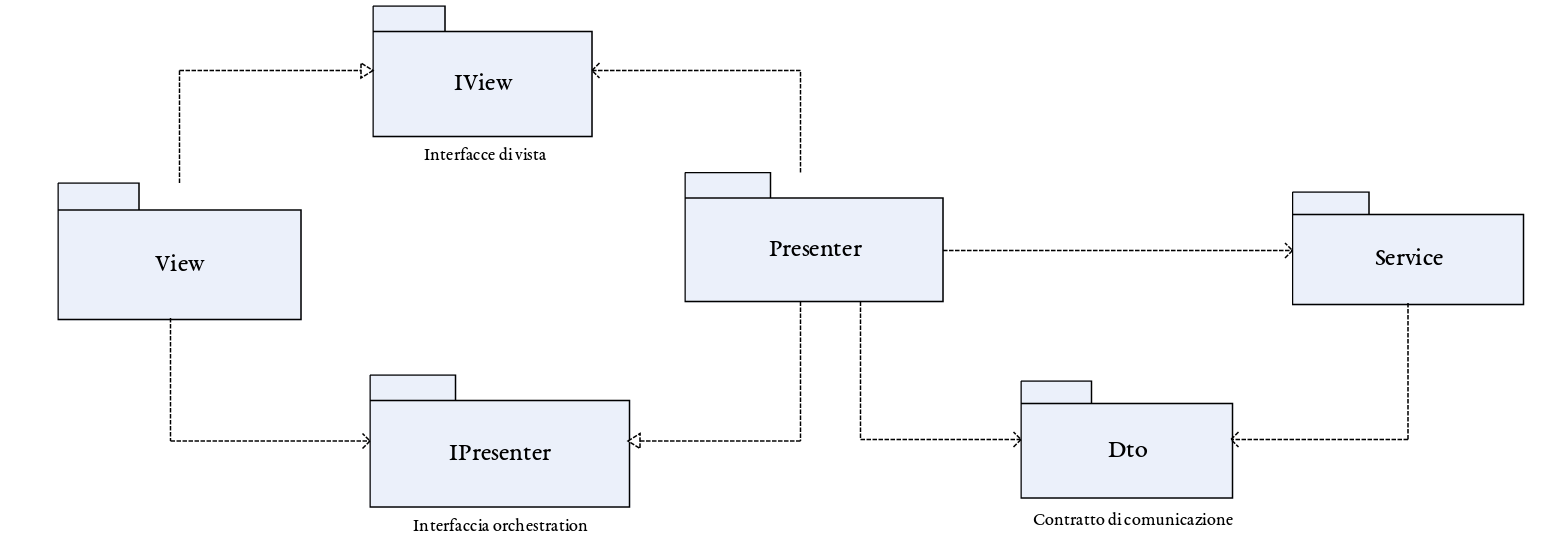
\includegraphics[width=13cm]{Chapters/pattern-front-end.png}
% \end{center}
% \caption{Diagramma dei package del front-end}
% \label{fig:f1} 
% \end{figure}

% I componenti grafici e il layout dell'applicazione si trovano nello strato \textit{View}. Non contengono logica sui dati, ma si limitano a ricevere i valori già pronti dallo strato \textit{Presenter}. \\
% Sebbene la logica applicativa sia definita altrove, i componenti grafici mantengono comunque una natura reattiva rispetto alle interazioni dell’utente: a questo scopo, sono state configurate le azioni in risposta agli eventi generati dall'utente. 

% Il \textit{Presenter} rappresenta lo strato di orchestrazione. Il funzionamento di questo strato si basa su un modello lineare: Il \textit{Presenter} intercetta i dati provenienti dalle interfacce di vista, converte tali dati in conformità con il contratto di comunicazione definito con il back-end e inoltra la richiesta. Successivamente riceve l'esito della chiamata dal server e, avvalendosi di un componente di mapping (mapper), adatta i dati ricevuti per restituirli alla \textit{View} pronti per la visualizzazione.

% Rispetto al classico modello MVP, il front-end non integra un \textit{modello di dominio} locale, ma si affida a uno specifico livello \textit{Service} che comunica direttamente con il \textit{Model} del back-end. Il modello espresso dal front-end è più precisamente un \textit{modello di presentazione}. \\
% \indent Più nel dettaglio, a livello di vista è stato adottato il \textit{pattern Composite} per organizzare i componenti grafici in una struttura ad albero. La motivazione che ha spinto a scegliere tale pattern risiede nella natura del toolkit grafico di JavaFX: la cui architettura si fonda nativamente su un grafo di nodi. \\
% \indent Il DTO, invece, rappresenta il \textit{modello dei dati} e, insieme all’albero dei componenti grafici, rappresenta l'unico altro modello definito all'interno del sottosistema.

% La ragione che ha indotto a non definire un \textit{modello di dominio} locale è di natura progettuale e di ottimizzazione: Il font-end è un client "leggero": riceve i dati dal server in formato DTO, li traduce e li mostra. Un livello \textit{domain} avrebbe duplicato quello del server senza aggiungere regole.

% % Gli strati di \textit{Adattamento} e \textit{Dati condivisi} non fanno parte di questo flusso, ma sono di supporto allo strato di \textit{Orchestrazione}. Il package \textit{Adattamento} traduce i dati in due sensi: costruisce le richieste da inviare al package \textit{Servizi} e converte le risposte in elementi visualizzabili, tramite interfacce che lo strato di \textit{Presentazione} implementa. Il package \textit{Dati condivisi} definisce il formato delle informazioni scambiate con il back-end ed è usato da  tutti gli strati che le maneggiano. Nessuno dei due è un passaggio obbligato per la richiesta: sono strumenti che l'orchestrazione impiega per trasformare correttamente i dati provenienti dall'interfaccia in richieste accettabili dal backend e le risposte del back-end in elementi che l’interfaccia può mostrare. \\ \\

% \subsection{Pattern MVP-\textit{Passive}}
% MVP-Passive è un modello architetturale comunemente utilizzato nello sviluppo di applicazioni mobili. Si tratta di un'evoluzione del modello MVC (\textit{Model-View-Controller}), incentrato su una separazione delle responsabilità che garantisce maggiore flessibilità e scalabilità.  \\
% \indent Il modello MVP è noto principalmente per semplificare la manutenibilità dell'applicazione, favorendone il miglioramento e la scalabilità nel tempo.

% Le proprietà principali di questo modello sono la rappresentazione dei dati e la definizione della logica di business dell'applicazione. È responsabile del recupero, dell'archiviazione e della manipolazione dei dati, nonché dell'applicazione delle regole aziendali. Il modello è indipendente dall'interfaccia utente e dovrebbe essere indipendente dall'implementazione specifica della vista (\textit{View}) e del presentatore (\textit{Presenter}).

% Il pattern si articola in tre componenti principali, come si nota dalla Figura 1.2.

% \begin{figure}[!ht] 
% \begin{center}
% 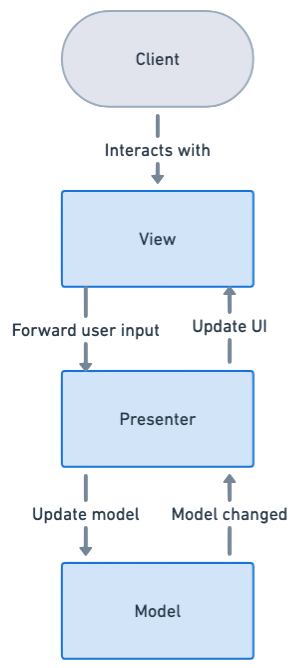
\includegraphics[width=4cm]{Chapters/pattern.png}
% \end{center}
% \caption{Pattern MVP-passive}
% \label{fig:f1} 
% \end{figure}

% \begin{quote}
% \begin{enumerate}[label=\textit{\arabic*}]
%    \item (\textit{View}): È responsabile della presentazione dei dati e dell'acquisizione dell'input dell'utente. È un \textit{componente passivo} che si basa sul \textit{Presenter} per aggiornare il proprio stato e gestire le interazioni dell'utente. \\
%    La vista in genere è costituita da elementi visivi come i componenti grafici dell'interfaccia utente (UI) e il layout dell'applicazione.
%    L'obiettivo principale di View è garantire che l'interfaccia utente sia reattiva, visivamente accattivante e facile da navigare.
  
%   \item (\textit{Presenter}): Il \textit{Presenter} funge da mediatore tra \textit{Model} e \textit{View}, orchestrando il flusso di dati e gestendo le interazioni dell'utente. È responsabile del recupero dei dati dal \textit{Model}, della loro elaborazione e dell'aggiornamento della \textit{View} di conseguenza. \\
%    Il \textit{Presenter} gestisce inoltre gli eventi utente dalla \textit{View}, come i clic sui pulsanti o le modifiche di input, attivaando azioni specifiche in base a questi eventi. \\
%    Separando gli aspetti della gestione dei dati (\textit{Model}) e dell'interfaccia utente (\textit{View}), \textit{Presenter} consente lo sviluppo di applicazioni più modulari, scalabili e manutenibili.

%   \item (\textit{Model}):  rappresenta i dati e la logica aziendale dell'applicazione, simile al modello in MVC. È responsabile dell'elaborazione, archiviazione e gestione dei dati e dell'implementazione di tutte le regole aziendali necessarie. Il modello non comunica direttamente con la vista o il presentatore.
% \end{enumerate} 
% \end{quote}

% Concludendo questo paragrafo sugli obiettivi che permette di raggiungere questo pattern, si possono certamente menzionare la separazione delle responsabilità tra i componenti, la manutenibilità e la scalabilità dell'applicazione; proprietà fondamentali che consentono di soddisfare le richieste in continua evoluzione da parte dei clienti. \\
% \indent Come esemplificato da molte piattaforme, il modello può essere integrato perfettamente in vari strumenti e metodologie di sviluppo, consolidando ulteriormente la sua rilevanza e importanza nel mondo dello sviluppo di applicazioni.

% % \begin{center}
% % 	\vspace*{-3em}
% % \def\arraystretch{2.0}
% % \begin{tabular}{|p{0.2\linewidth}|p{0.8\linewidth}|}
% % \hline
% % \textbf{Strato} & \textbf{Descrizione} \\
% % \hline 
% % \texttt{Interfaccia utente} & Lo strato \texttt{Interfaccia grafica} raccoglie la descrizione dei componenti grafici dell'applicazione, definita per mezzo di file FXML. Ogni file è associato a un controller, cioè a una classe dello strato di \texttt{Presentazione} che ne definisce il comportamento in risposta alle interazioni dell’utente  \\
% % \hline
% % \texttt{Presentazione} & Lo strato di \texttt{Presentazione} raccoglie le classi associate ai componenti grafici dell’interfaccia, cioè i controller dei file FXML. Le classi non sono slegate tra loro: si inseriscono nella struttura ad albero fornita dallo strato di \texttt{Base}, che riflette la composizione gerarchica dei componenti descritti dai file FXML. \\ 
% % \hline
% % \texttt{Base} & Data la natura gerarchica delle interfacce grafiche, lo strato di \texttt{Base} adotta il pattern \textit{Composite}: ogni vista è composta da componenti, a loro volta composti da altri componenti. Il legame è una composizione ricorsiva. Questo ha permesso di semplificre la gestione del ciclo di vita degli oggetti: quando una vista viene rimossa, vengono rilasciati anche tutti i componenti che la compongono. \\
% % \hline
% % \texttt{Orchestrazione} & Lo strato di \texttt{Orchestrazione} coordina il percorso dei dati tra l’interfaccia grafica e lo strato dei \texttt{Servizi}, nei due sensi. Ogni richiesta originata dall’utente raggiunge questo strato, che si avvale dello strato di \texttt{Adattamento} per costruire una richiesta in un formato comprensibile al back-end e la inoltra al servizio competente. In modo analogo, ogni risposta ricevuta dal back-end viene affidata allo strato di \texttt{Adattamento}, che la converte in elementi visualizzabili dall’interfaccia.
% % \\
% % \end{tabular} 
% % \end{center}

% % \begin{center}
% % 	\vspace*{-3em}
% % \def\arraystretch{2.0}
% % \begin{tabular}{|p{0.2\linewidth}|p{0.8\linewidth}|}
% % \texttt{Adattamento} & Lo strato di \texttt{Adattamento} traduce i dati nei due sensi. Nel verso dell’invio, converte le informazioni provenienti dall’interfaccia in richieste in un formato comprensibile al back-end. Nel verso della ricezione, converte le risposte del back-end in elementi visualizzabili dall’interfaccia. Lo strato non dipende dai componenti grafici concreti: opera su interfacce che lo strato di \texttt{Presentazione} implementa, così la logica di traduzione resta indipendente dalla grafica.\\ 
% % \hline
% % \texttt{Dati Condivisi} & Lo strato \texttt{Dati condivisi} definisce il contratto di comunicazione con il back-end. Raccoglie le classi DTO, usate come formato standard di scambio delle informazioni. \\
% % \hline
% % \texttt{Servizi} & Lo strato dei \texttt{Servizi} gestisce la comunicazione con il back-end: effettua le richieste HTTP e riceve le relative risposte. È l’unico strato a conoscere il protocollo di trasporto, e questo isola il resto del sottosistema dai dettagli della comunicazione. Le richieste e le risposte sono rappresentate da oggetti DTO, che i servizi ricevono dallo strato di \texttt{Orchestrazione} e a cui restituiscono i risultati. \\
% % \hline
% % \end{tabular} \\
% % \end{center} 

% \subsection{Back-end}
% L'architettura del back-end adotta un modello di stratificazione basato sul pattern \textit{Controller-Service-Repository}, scelto specificamente per garantire una netta separazione delle responsabilità tra i diversi componenti del sistema. 

% La suddivisione dei ruoli si articola come in figura

% \begin{figure}[!ht] 
% \begin{center}
% 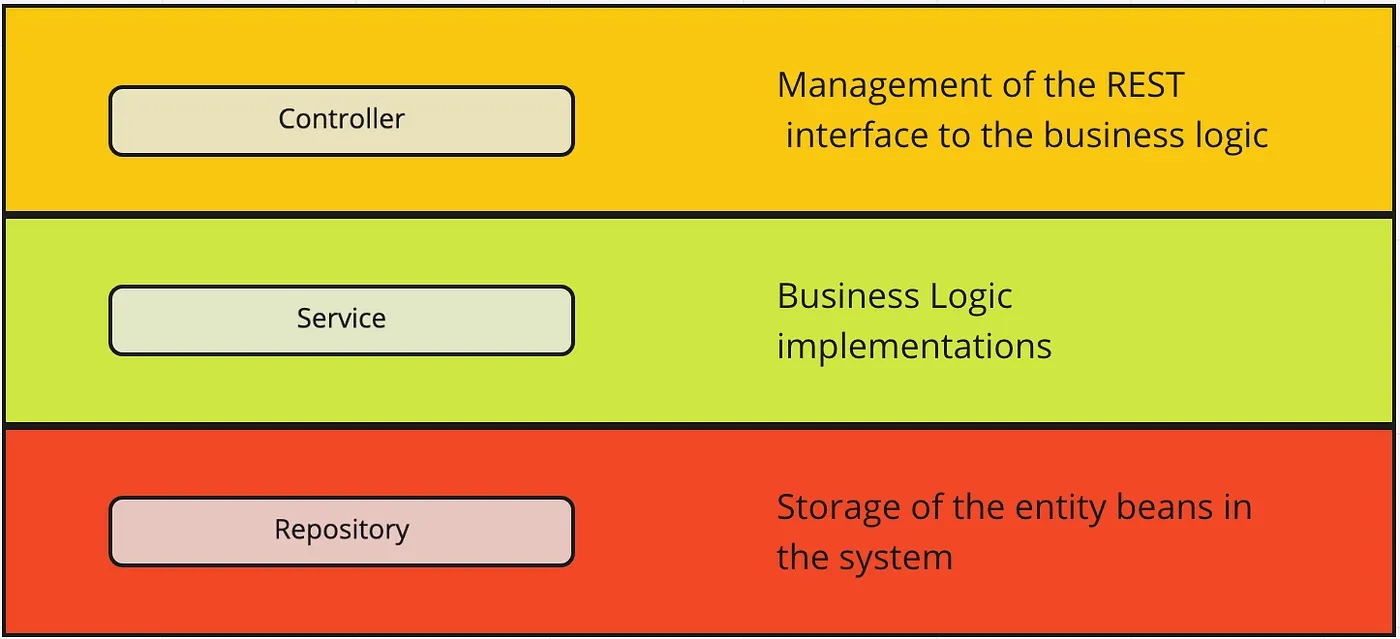
\includegraphics[width=10cm]{Chapters/controller.jpeg}
% \end{center}
% \caption{Back-end}
% \label{fig:f1} 
% \end{figure}

% \begin{quote}
% \begin{enumerate}[label=\textit{\arabic*}]
%    \item (\textit{Controller}): ha il solo compito di esporre le funzionalità del sistema, rendendole accessibili a entità esterne, come un'interfaccia utente.
  
%   \item (\textit{Service}): Questo livello centrale è il cuore del sistema e contiene tutta la logica di business. Se questa logica ha bisogno di leggere o salvare dati, si interfaccia con il Repository. Per accedere alla logica di business, invece, è necessario passare tramite il Controller.

%   \item (\textit{Repository}): Questo livello ha la responsabilità esclusiva di salvare e recuperare un determinato insieme di dati.
% \end{enumerate} 
% \end{quote}

% L'adozione di questo pattern apporta molteplici benefici in termini di manutenibilità e scalabilità del software:

% \begin{quote}
% \begin{enumerate}[label=\textit{\arabic*}]
%    \item (\textit{Riusabilità}):la logica applicativa risiede in un unico punto e può essere invocata in modo flessibile da molteplici endpoint.
  
%   \item (\textit{Indipendenza dei componenti}):ogni livello può evolvere e subire modifiche senza impattare sugli altri (garantendo, in particolare, il totale disaccoppiamento tra il back-end e il front-end).

%   \item (\textit{Testabilità}): l'isolamento dei componenti service consente di effettuare unit test mirati, sostituendo i repository con oggetti mock per simulare il comportamento della base di dati.
% \end{enumerate} 
% \end{quote}

% \subsubsection{Repository pattern}
% Per la gestione dell'accesso ai dati è stato adottato il Repository Pattern. L'obiettivo di questo pattern è fornire all'applicazione un'interfaccia astratta e generica per interagire con il layer dei dati, rendendo l'architettura indipendente dai dettagli implementativi (che si tratti di un database locale o di un'API remota).

% I metodi si basano sulle operazioni standard \textit{CRUD} (Create, Read, Update, Delete). Ciascuna entità di dominio dispone del proprio repository dedicato: un componente che si comporta analogamente a una collezione in memoria, consentendo ai service di effettuare ricerche, salvataggi ed eliminazioni senza dover conoscere le logiche sottostanti di memorizzazione. \\ 
% \indent In questo modo, la logica di business rimane rigorosamente separata dai dettagli di persistenza (query SQL, tabelle e connessioni), garantendo che eventuali modifiche al sistema di archiviazione dei dati non richiedano alcun intervento sui service.

% \section{Stratificazione dei sottosistemi}
% I due sottosistemi sono stati ulteriormente decomposti in parti più piccole in base alle responsabilità che ricoprono; come si evince dalla Figura 3.5 e dalla Figura 3.6 riportate qui di seguito.

% \begin{figure}[!ht] 
% \begin{center}
% 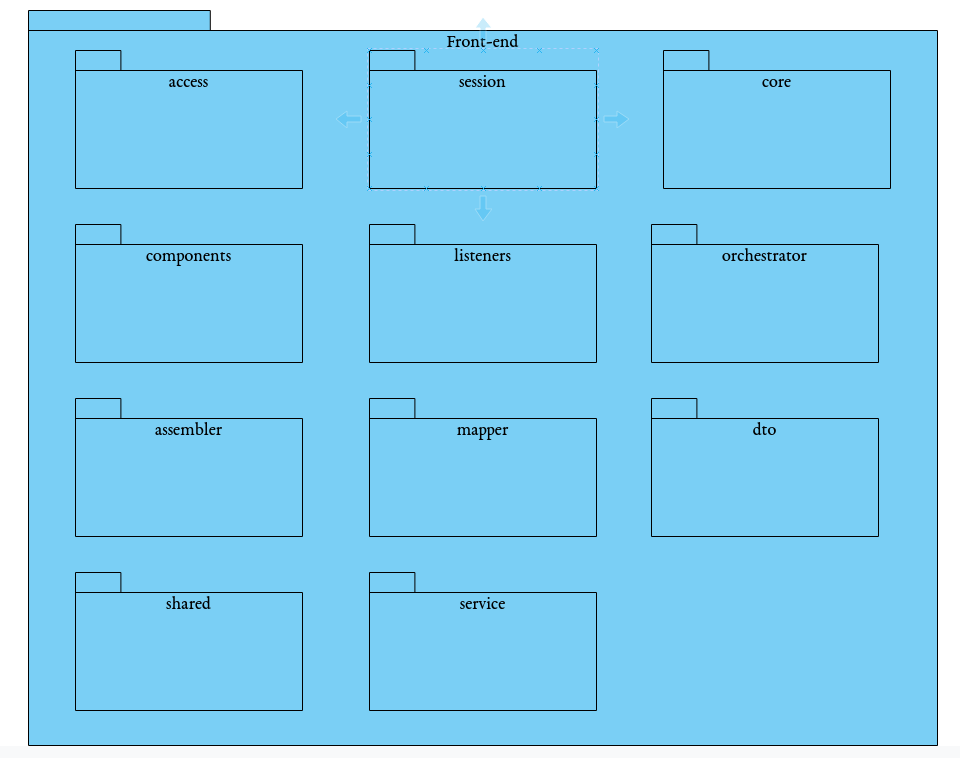
\includegraphics[width=8cm]{Chapters/front-end.png}
% \end{center}
% \caption{Front-end}
% \label{fig:f1} 
% \end{figure}

% \begin{figure}[!ht] 
% \begin{center}
% 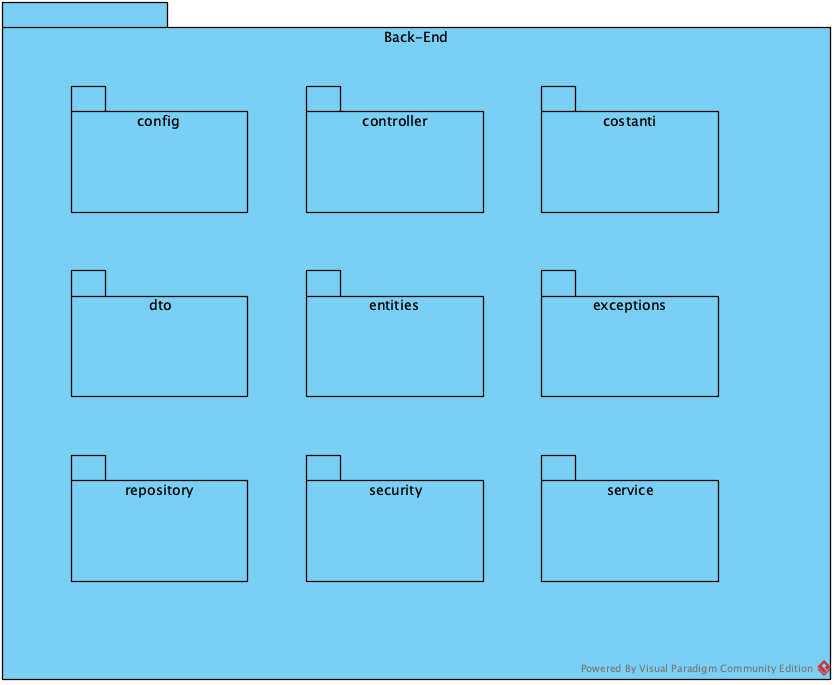
\includegraphics[width=8cm]{Chapters/Immagine.png}
% \end{center}
% \caption{Back-end}
% \label{fig:f1} 
% \end{figure}

% \section{Descrizione delle scelte tecnologiche adottate}

% \subsection{Spring Boot}
% Per il back-end si è scelto Spring Boot, il framework più diffuso per lo sviluppo di servizi REST in Java. Spring Boot segue il paradigma convention over configuration: fornisce una configurazione predefinita ragionevole per gli aspetti più comuni (server web integrato, connessione al database, conversione JSON), così gli sviluppatori devono specificare solo ciò che si discosta dallo standard. \\ 
% \indent Questo riduce il codice di configurazione e il numero di decisioni da prendere, senza perdere flessibilità: ogni impostazione predefinita può essere sovrascritta quando serve. 

% Spring offre inoltre la dependency injection: controller, service e repository vengono creati dal framework e collegati tra loro automaticamente, il che rende i componenti indipendenti e facili da testare. \\
% \indent Infine il suo ecosistema mette a disposizione moduli già integrati per tutte le esigenze del progetto: Spring Web per le API REST, Spring Data JPA per l'accesso al database, Spring Security per l'autenticazione e i permessi, Jakarta Validation per il controllo dei dati in ingresso. Usare soluzioni standard e collaudate, invece di scriverle da zero, ha consentito di focalizzare gli sforzi sulla logica di business, riducendo gli errori soprattutto in un ambito delicato come la sicurezza.  

% \subsection{Docker}
% È stato usato per automatizzare la distribuzione del back-end di BugBoard26 sotto forma di container, cioè un pacchetto contenente l'applicazione insieme a tutto ciò che le serve per funzionare (il runtime Java e le librerie). \\
% \indent Il container si comporta allo stesso modo su qualsiasi macchina, dal computer di sviluppo a un server nel cloud, ed elimina i problemi di installazione e configurazione dell'ambiente. Il Dockerfile è di tipo multi-stage: l'applicazione viene compilata in un'immagine con il JDK e Maven, mentre l'immagine finale contiene solo il runtime Java e l'applicazione, quindi è più eggera e non include strumenti di compilazione. Infine con Docker Compose il back-end e il database MySQL si avviano insieme con un unico comando: il back-end parte solo quando il database è pronto, e i dati vengono conservati in un volume, così non si perdono quando i container vengono riavviati. 

% \subsection{Libreria JavaFX}
% Per questa applicazione desktop è stato utilizzato JavaFX come toolkit grafico. Tra i suoi vantaggi merita di essere menzionata la gestione del layout, che permette di separarlo dal codice. Il layout si trova in file FXML, che descrivono in modo dichiarativo i componenti grafici dell’applicazione. Ogni file è associato a un controller, cioè a una classe che ne definisce il comportamento in risposta alle interazioni dell’utente: senza controller l’interfaccia è priva di comportamento. \\\
% \indent L’aspetto grafico è definito in fogli di stile CSS e si applica ai componenti tramite classi di stile, senza modificare il codice. Infine, lo stesso codice Java può essere eseguito su più piattaforme, come Windows, macOS e Linux.

% \subsection{Ambienti di sviluppo utilizzati}
% Il sistema è stato sviluppato in Java, usato sia per il back-end sia per il front-end. Come ambiente di sviluppo è stato usato IntelliJ IDEA di JetBrains. \\
% \indent Java 21 è stata la versione utilizzati da entrambi gli applicaativi. Nel back-end è stato usato con il framework Spring Boot, nel front-end con la libreria JavaFX. Usare lo stesso linguaggio nei due componenti ha semplificato lo sviluppo e la collaborazione tra i membri del gruppo.

\section{Diagramma delle classi di design}
I diagrammi qui descritti sono quelli che effettivamente rappresentano il sistema sviluppato. 
Per una maggiore leggibilità, si è scelto di suddividere i diagrammi in base al sottosistema 
di appartenenza. \\
\indent I diagrammi delle classi riportati afferiscono a un diverso livello di dettaglio: 
per la parte front-end si è scelto di dare maggiore importanza alle interazioni e ai flussi 
di comunicazione tra i diversi livelli dell'architettura, evitando di fare un "dump" speculare di tutto il codice sorgente e privilegiando solo la struttura logica, la separazione delle responsabilità e il flusso delle dipendenze tra i diversi livelli. \\
\indent Per quanto riguarda il lato back-end, il relativo modello di dominio e la descrizione delle
scelte di design adottate saranno trattati 
nella sezione dedicata. 

\subsection{Front-end}

Qui di seguito è illustrato il \textit{modello di presentazione} 
(front-end), evidenziando la struttura gerarchica dei componenti grafici.

\begin{figure}[!ht]
    \centering
    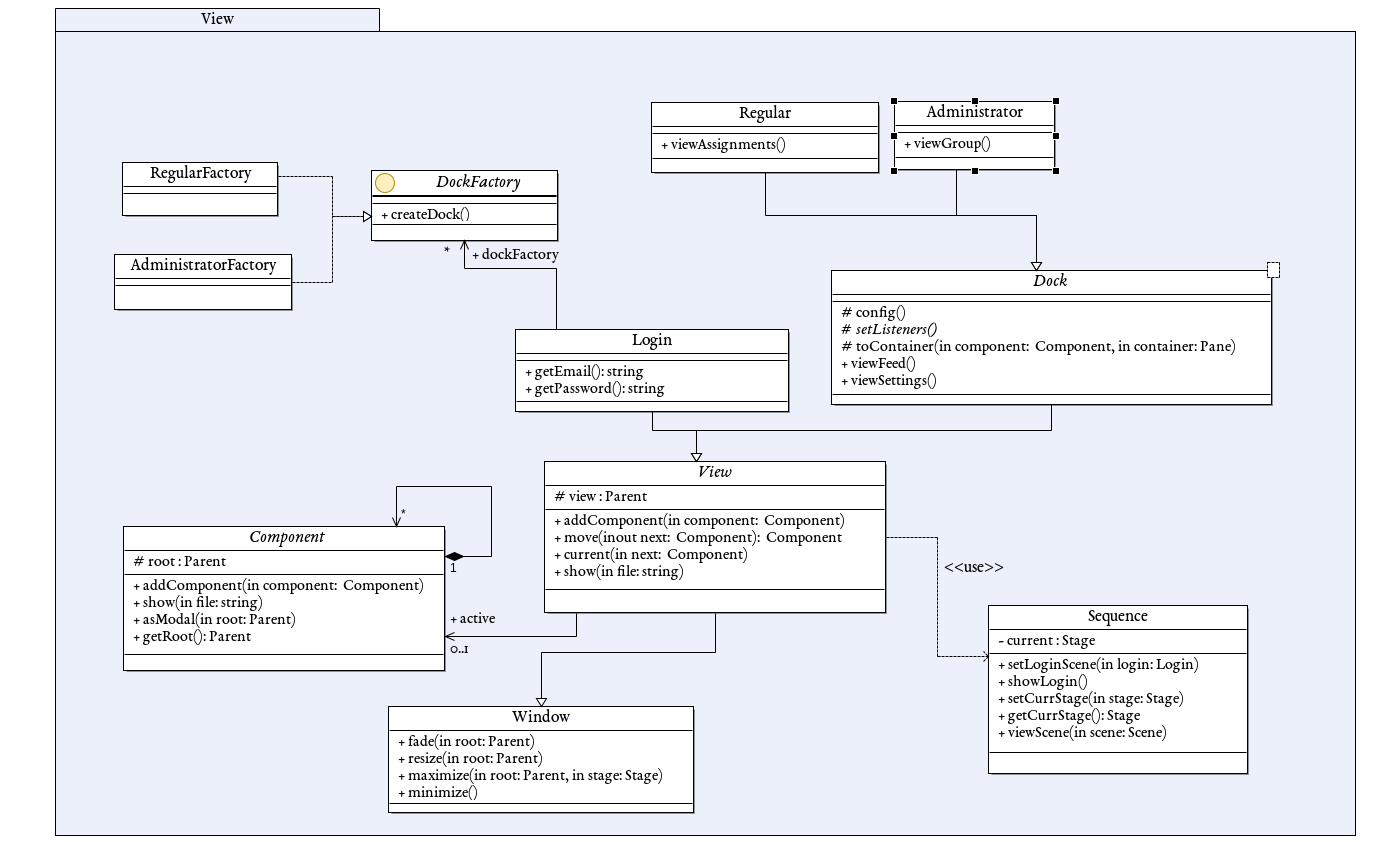
\includegraphics[width=\linewidth]{Chapters/View.png}
    \caption{Livello View}
    \label{fig:f1}
  \end{figure}

  \newpage

Sempre in corrispondenza del livello \textit{View} si trovano le seguenti classi che si estendono solo orizzontalmente secondo le proprietà della composizione ricorsiva.

\begin{figure}[!ht] 
\begin{center}
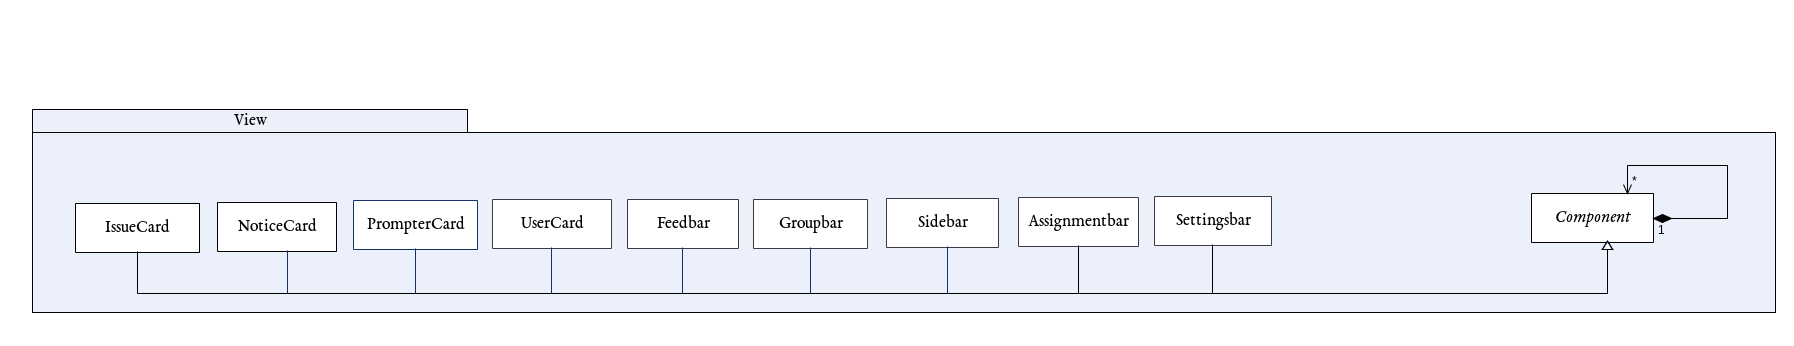
\includegraphics[width=\linewidth]{Chapters/composite.png}
\end{center}
\caption{Pattern \textit{Composite}}
\label{fig:f1} 
\end{figure}

La struttura di questo pattern garantisce un'elevata estendibilità: qualora fosse necessario introdurre una nuova tipologia di componente grafico (es. la pagina della Dashboard), distinta da quelle già presenti nel sistema, è sufficiente definire una nuova classe concreta che estenda \textit{Component}. Grazie alla condivisione della classe astratta in comune, il componente grafico acquisisce immediatamente la capacità di inserirsi in qualsiasi punto della catena di composizione a runtime. \\
\indent Infine, è possibile arricchire  l'oggetto base con la nuova funzionalità senza dover modificare né la classe \textit{Component} e né i componenti preesistenti, aderendo rigorosamente al principio Open/Closed. \\
\indent Un altro vantaggio della composizione ricorsiva risiede nella gestione efficiente del ciclo di vita degli oggetti. Infatti, quando una vista viene rimossa, vengono rilasciati anche tutti i componenti che la compongono, semplificando enormente il lavoro da parte del Garbage Collector.

Le classi \texttt{Feedbar}, \texttt{Groupbar}, \texttt{Sidebar}, 
\texttt{Assignmentbar} e \texttt{Settingsbar} sono componenti principali: contengono altri componenti, come le card e i moduli, secondo la composizione ricorsiva di 
\texttt{Component}. Sono loro a inserire nel proprio contenitore 
i componenti che il livello \texttt{Presenter} restituisce già popolati con i dati 
provenienti dal back-end. La struttura uniforme del pattern permette inoltre 
che uno stesso componente sia, a seconda del punto dell’albero in cui si 
trova, contenitore di altri componenti oppure foglia.


\indent È bene notare, che i componenti grafici sono stati 
rappresentati da classi spogliate sia dei metodi sia degli attributi. 
Il fine ultimo del diagramma è comunicare come il pattern \textit{Composite}
 organizzi i componenti grafici all'interno di un albero, il quale 
 riflette altresì la composizione gerarchica dei componenti descritti 
 dai file FXML. \\
 \indent Per tale motivo, per evitare di appesantire il diagramma, alcune classi sono state omesse;
 approfittando del grande vantaggio di seguire lo stesso schema di quelle riportate,
  la loro aggiunta non avrebbe aumentato la comprensione.

\begin{figure}[!ht] 
\begin{center}
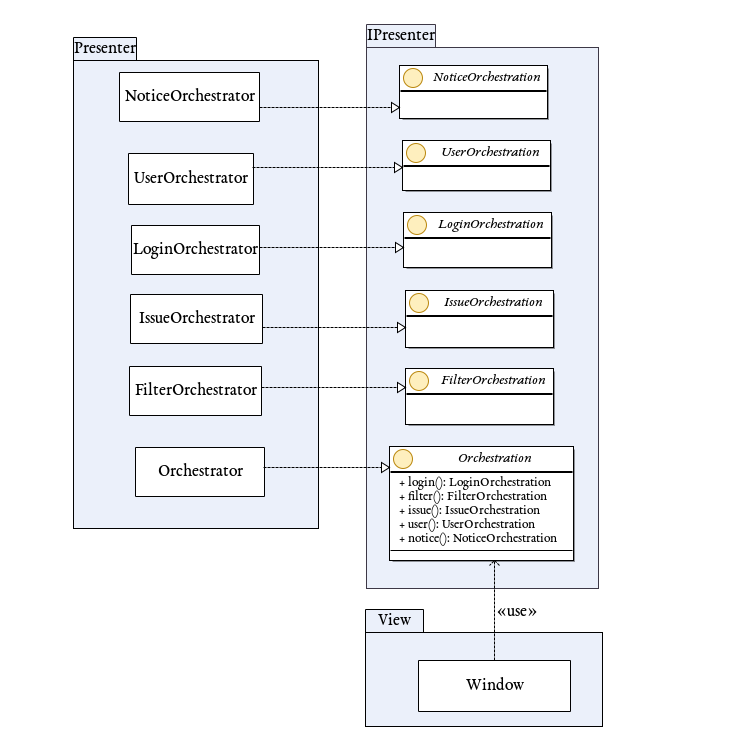
\includegraphics[width=10cm]{Chapters/presenter.png}
\end{center}
\caption{Livello View e livello IPresenter}
\label{fig:f1} 
\end{figure}

La figura mostra il punto di contatto tra il livello \texttt{View} e il livello
 \texttt{IPresenter}. La classe \texttt{Window}, radice della gerarchia di 
 \texttt{View} e di \texttt{Component}, custodisce un oggetto 
di tipo \texttt{Orchestration} che viene istanziato una sola volta all'avvio 
dell'applicazione. \\
\indent Tale scelta evita di propagare gli orchestratori lungo la catena dei 
costruttori che hanno come termine le viste concrete. Inoltre, ogni classe appartenente 
alla gerarchia di \texttt{Window} è 
in grado di invocare l'orchestratore di cui ha bisogno, senza riferirsi agli oggetti
 dello strato \texttt{Presenter}.

\begin{figure}[!ht] 
\begin{center}
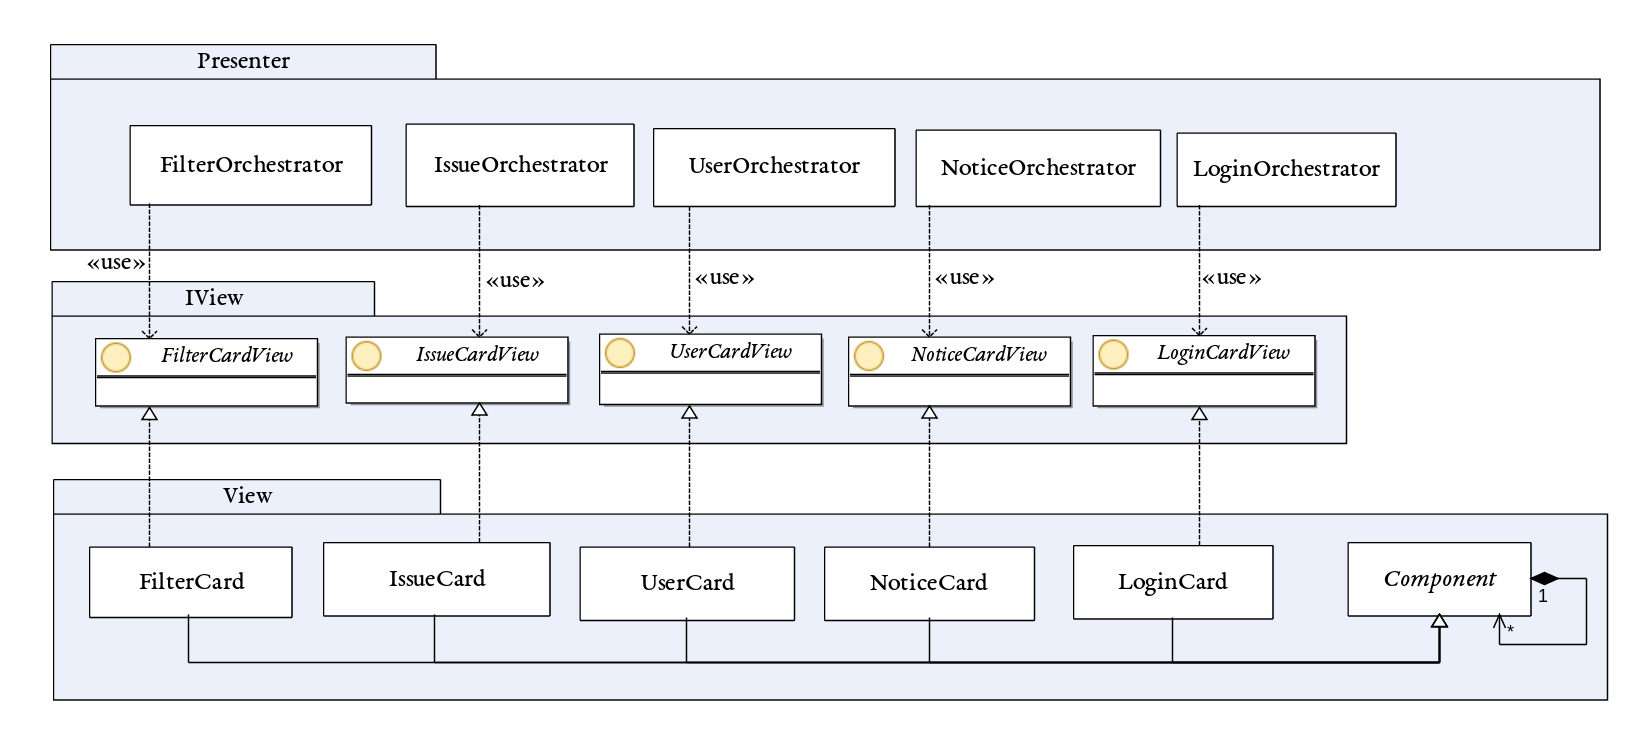
\includegraphics[width=\linewidth]{Chapters/IView.png}
\end{center}
\caption{Collegamento tra il livello \texttt{Presenter}, il livello \texttt{IView} e \texttt{View}}
\label{fig:f1} 
\end{figure}

\newpage

Questo diagramna chiarisce il motivo di custodire all'interno della classe 
\texttt{Window}
un oggetto di tipo \texttt{Orchestration}. Ogni card ha bisogno del proprio 
orchestratore 
per inviare i dati e riceverli, e la soluzione adottata evita di propagare gli oggetti
orchestratori lungo la catena di construttori. 

Nel diagramma sono riportate solo le classi a cui il \texttt{Presenter} accede 
tramite le interfacce del livello \texttt{IView}.
Le altre classi, come \texttt{Feedbar} e \texttt{Groupbar}, non sono 
accedute dal \texttt{Presenter}: sono loro a invocarne i contratti, attraverso 
il riferimento a \texttt{Orchestration} presente in \texttt{Window}, e 
a ricevere come risultato i dati già composti, come mostrato in Figura 4.3.

La figura mostra anche il meccanismo di comunicazione tra il livello 
\texttt{Presenter} e il livello \texttt{IView}.
Si prenda, a titolo di esempio, la classe 
\texttt{IssueCard}, che rappresenta sia una issue che si vuole creare sia una 
issue già esistente nel sistema. Si supponga che classe \texttt{Feedbar},
responsabile della visualizzazione e della creazione delle issue, invochi il
metodo \texttt{create()} di \texttt{IssueOrchestrator} tramite il riferimento
a \texttt{Orchestration}. \\
\indent Il flusso di esecuzione è il seguente: Come prima 
operazione, l'utente inserisce i valori relativi alla priorità, al titolo, 
alla tipologia e così via all’interno della card. L'oggetto con i campi 
compilati viene passato all'orchestratore che estrapola i campi, invocando 
i metodi dell'interfaccia, costruisce l'oggetto per il backend e lo invia. \\
\indent La risposta del back-end viene convertita dal \texttt{Mapper}
in una \texttt{IssueCard} che l’orchestrator 
restituisce alla \texttt{Feedbar} per la visualizzazione. 
\texttt{Assembler} e \texttt{Mapper}, che fanno parte del livello \texttt{Presenter}, 
sono descritti nella Figura 4.6.

Il livello \texttt{Presenter}, come specificato dal pattern, comunica con il back-end
mendiante il livello \texttt{Service} che rispecchia i servizi forniti dalla parte
back-end. La seguente figura illustra chiaramente questa situazione.

\newpage

\begin{figure}[!ht] 
\begin{center}
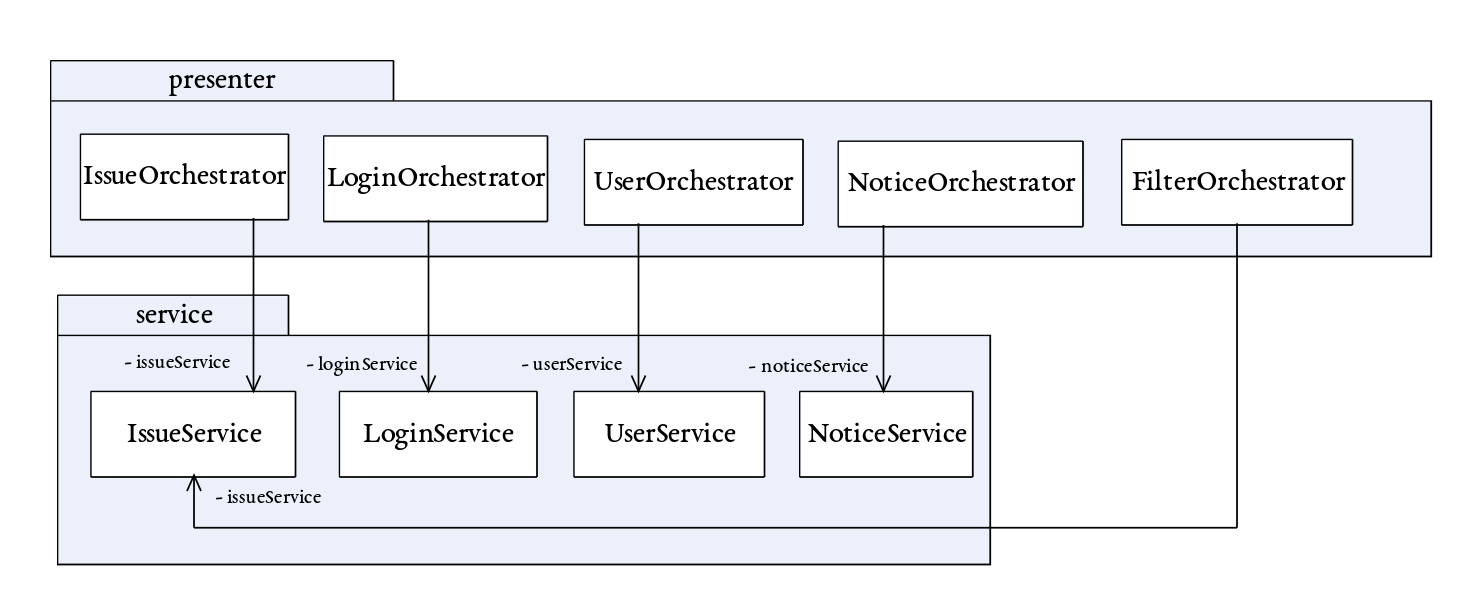
\includegraphics[width=\linewidth]{Chapters/presenter_service.png}
\end{center}
\caption{Collegamento tra il livello \texttt{Presenter} e il livello \texttt{Service}}
\label{fig:f1} 
\end{figure}

La situazione rappresentata dalla Figura 4.6 descrive due momenti: il momento dell'impacchettamento 
dei dati per essere inviati al server, e il momento della conversione dei dati
ricevuti dal server stesso. \\
\indent Front-end e Back-end comunicano 
attraverso un contratto di comunicazione di informazioni, rappresentato 
dalle classi DTO. Gli orchestratori assemblano i dati provenienti dai 
componenti grafici in pacchetti di dati in formato DTO. L'oggetto prodotto 
viene poi passato all'ultimo livello (\textit{Service}) che è il vero e 
proprio responsabile dell'invio dei dati.
I dati ricevuti dal server vengono successivamente convertiti nel componente grafico corretto.

\begin{figure}[!ht] 
\begin{center}
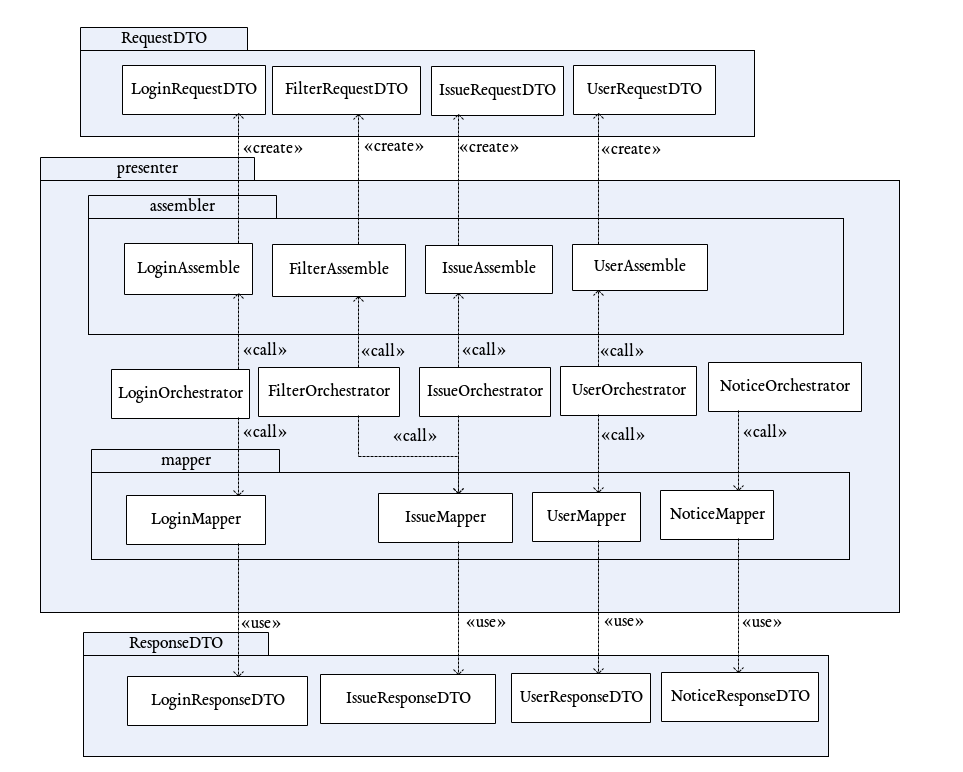
\includegraphics[width=12cm]{Chapters/assembler-mapper.png}
\end{center}
\caption{Collegamento tra il livello \texttt{Presenter} e il livello \texttt{Dto}}
\label{fig:f1} 
\end{figure}

\newpage

L'ultima figura mostra l'ultimo punto di contatto dell'architettura. In tale situazione
le classi \texttt{service} si servono dei contratti di comunicazione che definisco il
formato di scambio dati con il back-end. Le classi del package \texttt{service} non conoscono 
il \texttt{Presenter} né la \texttt{View}: ricevono dall’orchestratore un oggetto di tipo
\texttt{RequestDTO}, con cui costruiscono la richiesta HTTP da inviare al server. \\
\indent La risposta del server viene convertita in un oggetto di tipo \texttt{ResponseDTO}, che il servizio restituisce 
all’orchestrator; come descritto nella Figura 1.11, questi lo passa al mapper, che lo converte nel 
componente grafico corretto. \\
\indent La dipendenza \textit{«use»} indica che le classi del package \texttt{service} usano l’oggetto di tipo \texttt{RequestDTO} 
ricevuto come parametro. La creazione degli oggetti di tipo \texttt{ResponseDTO} è espressa invece dalla 
dipendenza \textit{«create»}.

\begin{figure}[!ht] 
\begin{center}
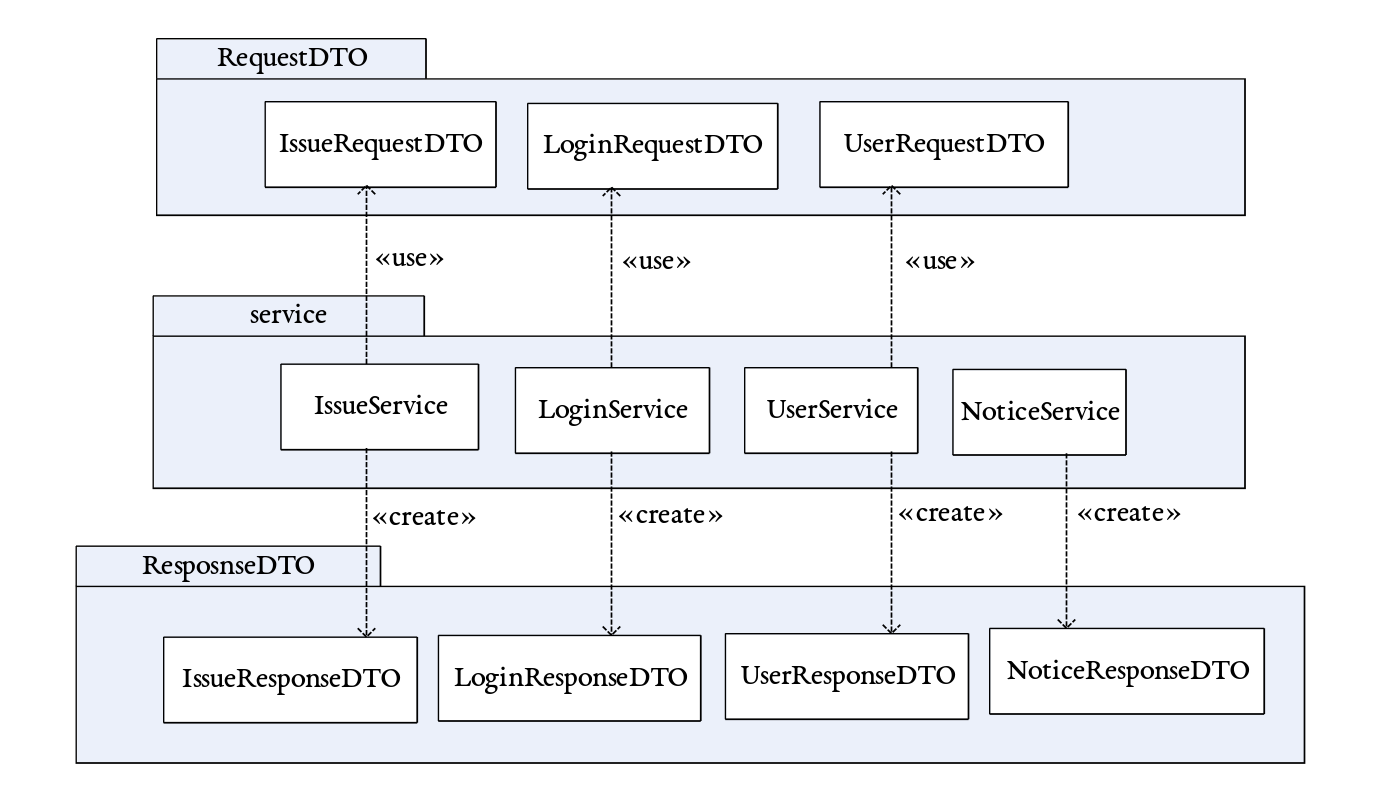
\includegraphics[width=\linewidth]{Chapters/service_dto.png}
\end{center}
\caption{Collegamento tra il livello \texttt{Service} e il livello \texttt{dto}}
\label{fig:f1} 
\end{figure}

\subsection{Back-end}
La presente sezione descrive le principali scelte fatte nel progettare
il codice del back-end e il motivo di ognuna di esse.
Qui di seguito è illustrato il \textit{modello di dominio}.

\begin{figure}[!ht] 
\begin{center}
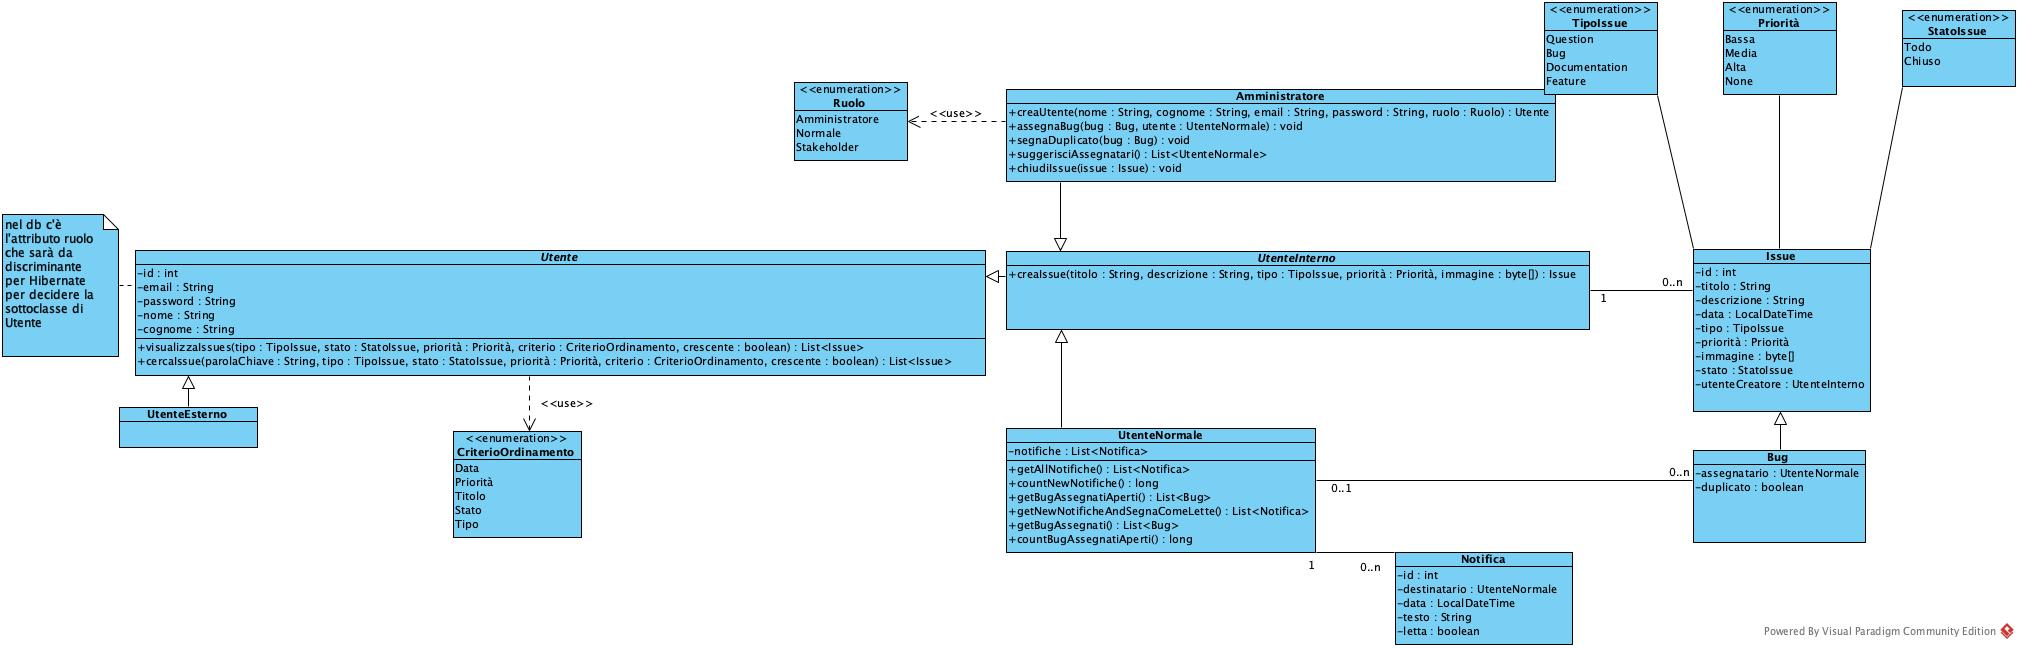
\includegraphics[width=\linewidth]{Chapters/modello di dominio.jpg}
\end{center}
\caption{Modello di dominio}
\label{fig:f1} 
\end{figure}

\subsubsection{I ruoli come sottoclassi}
I ruoli degli utenti non sono un campo da controllare con degli if, ma sottoclassi 
di Utente: Amministratore e UtenteNormale (entrambi UtenteInterno) e UtenteEsterno
 (lo stakeholder, che può solo consultare le issue). \\
 \indent In questo modo i permessi 
 diventano tipi: il creatore di un'issue è di tipo UtenteInterno, l'assegnatario di 
 un bug e il destinatario di una notifica sono di tipo UtenteNormale. È quindi il 
 compilatore a impedire, per esempio, che uno stakeholder risulti autore di un'issue, 
 senza controlli sparsi nel codice. 

 \subsubsection{Bug come sottoclasse di Issue }
 Solo i bug si possono assegnare e segnare come duplicati, quindi Bug è 
 una sottoclasse di Issue con i suoi campi in più (assegnatario e duplicato). \\
 \indent I metodi assegnaBug e segnaDuplicato ricevono un Bug: chiamarli su una question
  o una feature non è possibile. Il metodo creaIssue crea un Bug se e solo se 
  il tipo indicato è BUG. 

\subsubsection{Stato, priorità e duplicati }
 StatoIssue (TODO, CHIUSO) sta su Issue e non solo su Bug, perché 
 ogni issue nasce TODO e può essere chiusa. \\
\indent Priorita ha un valore NONE per "priorità non indicata" 
invece di null: così la priorità è sempre valorizzata, e filtrare o ordinare 
per priorità non richiede di gestire i valori mancanti. \\
\indent Il bug duplicato è indicato con un semplice valore vero/falso, senza un 
riferimento al bug originale: il requisito chiede solo di segnarlo e chiuderlo,
 e un riferimento in più avrebbe aggiunto vincoli senza una funzionalità che li usasse. 

\subsubsection{ Organizzazione dei service}
I service sono divisi in due gruppi: 

- Service "attore" (AmministratoreService, UtenteInternoService, UtenteNormaleService, UtenteService): contengono le operazioni del class diagram, 
cioè le azioni che un utente compie, raggruppate per la classe che le esegue. 

- Service "di entità" (IssueService, BugService, NotificaService): contengono le operazioni 
di base e di supporto, che non sono azioni di un utente ma vengono usate dai service attore. 

La regola è: se un utente la compie come azione va nel service attore, se è un effetto 
di un'altra azione va nel service di entità. Per esempio creaNotifica sta in NotificaService 
e non in AmministratoreService, perché nessun utente "crea una notifica": la notifica è un 
effetto di assegnaBug, segnaDuplicato e chiudiIssue, che la riusano tutti. Così il codice 
segue il class diagram, e ogni service attore corrisponde a una sua classe. 

I service inoltre non controllano i permessi: non ricevono un parametro Amministratore 
per sapere chi li sta chiamando. I permessi si controllano prima, sugli endpoint (vedi 3c.4).
 L'utente loggato arriva al service solo quando è un dato dell'operazione, per esempio il 
 creatore di un'issue in creaIssue.

\subsubsection{DTO e validazione}
I controller non restituiscono mai le entità, ma dei DTO (Data Transfer Object): semplici 
record Java con i soli campi da mandare al client. Le entità non sono adatte a essere 
trasformate in JSON: 

- Utente contiene l'hash della password, che non deve uscire dal server. 

- Alcune relazioni sono circolari (un utente ha le sue notifiche, ogni notifica 
ha il suo destinatario) e la conversione in JSON non finirebbe mai. 

- Il JSON è il contratto con il front-end: con i DTO un cambiamento nel 
database non lo rompe. 

Anche i dati in ingresso arrivano come DTO (per esempio CreaIssueRequest) e 
vengono controllati su due livelli. I controlli di formato (campi obbligatori, 
lunghezze massime uguali a quelle delle colonne, formato dell'email, dimensione 
dell'immagine) sono annotazioni sui DTO, come @NotBlank e @Size, e rifiutano la 
richiesta prima che arrivi alla logica. Le regole di business (email già in uso, 
bug già chiuso, bug già duplicato) sono invece nei service.

\subsubsection{Sicurezza}
L'autenticazione usa Spring Security con la sessione HTTP: dopo il 
login il server ricorda l'utente e il client riceve un cookie da allegare 
alle richieste successive. All'inizio avevamo valutato i token JWT, ma li 
abbiamo scartati perché più complessi da gestire (firma, scadenza, rinnovo) 
senza vantaggi per un sistema con un solo back-end e un solo client. 
Le password sono salvate solo come hash BCrypt, e al login un'email 
inesistente e una password sbagliata danno lo stesso errore, per non 
rivelare quali email sono registrate. 

I permessi sono dichiarati con @PreAuthorize su ogni endpoint 
(per esempio hasRole('AMMINISTRATORE') per assegnare un bug): l'attore del 
class diagram diventa il ruolo richiesto dall'endpoint. Tutto tranne il login 
richiede di essere autenticati, quindi se ci si dimentica un'annotazione 
l'endpoint resta comunque chiuso a chi non ha fatto l'accesso. 

\subsubsection{Gestione degli errori}
I service segnalano i problemi lanciando eccezioni, e un'unica classe, 
GlobalExceptionHandler, le trasforma nella risposta HTTP giusta: 400 per dati non validi, 
401 per credenziali sbagliate, 404 per una risorsa inesistente, 409 per un'operazione in 
conflitto con lo stato attuale (per esempio assegnare un bug chiuso). Gli errori 401 e 
403 generati da Spring Security usano lo stesso formato. In questo modo i controller 
non hanno try/catch e il client riceve sempre errori con la stessa struttura, con un 
messaggio che può mostrare all'utente. 

\subsubsection{Regole di business}
Dove i requisiti lasciavano margine abbiamo deciso noi il comportamento: 

- creaUtente: l'email viene salvata in minuscolo e deve essere unica, 
per evitare due account con la stessa email scritta in modo diverso. 

- assegnaBug: un bug chiuso non si può assegnare. Se il bug passa 
da un utente a un altro, ricevono la notifica sia il nuovo sia il 
vecchio assegnatario. 

- suggerisciAssegnatari: gli utenti sono ordinati per numero di 
bug ancora aperti (TODO) assegnati, dal meno al più carico. 

- segnaDuplicato: un bug già segnato come duplicato non si può 
segnare di nuovo; il bug viene chiuso e l'assegnatario avvisato. 

- chiudiIssue: è riservata all'amministratore, e chiudere 
un'issue già chiusa non dà errore. 

Le operazioni che fanno più scritture insieme, come assegnaBug 
(aggiorna il bug e crea le notifiche), sono @Transactional: o riescono 
tutte o nessuna, così non restano notifiche di un'assegnazione mai avvenuta. 

\subsubsection{Filtri e ordinamenti nel database}
La vista delle issue permette di filtrare e ordinare per vari criteri. 
Invece di caricare tutte le issue e ordinarle in Java, abbiamo scritto 
le query in IssueRepository: una parte comune con i filtri e un ORDER BY 
diverso per ogni criterio e direzione. Il service sceglie la query giusta 
con uno switch. Così è il database, che lo fa in modo efficiente, a filtrare e 
ordinare, e al back-end arrivano solo le issue richieste. 

\section{Schema di persistenza dei dati}
In questa sezione descriviamo come Bugboard26 conserva i propri dati: 
quale database abbiamo scelto, come è fatto lo schema, come le classi del 
class diagram sono state trasformate in tabelle e come lo schema viene creato 
e aggiornato nel tempo. 

\subsection{Database e gestione dello schema}
Per la persistenza abbiamo usato MySQL 8, un database relazionale. I 
dati di Bugboard26 sono strutturati e collegati tra loro (un'issue ha un 
autore, un bug ha un assegnatario, una notifica ha un destinatario), quindi 
il modello relazionale, con le sue chiavi esterne e le transazioni, è quello più adatto. 

Lo schema è stato progettato con MySQL Workbench, disegnando prima il 
modello ER e generando poi automaticamente lo script SQL di creazione delle 
tabelle (forward engineering). 

Il back-end accede al database tramite JPA (con Hibernate come implementazione) e 
Spring Data JPA: le classi del dominio sono entità mappate sulle tabelle, e i 
repository offrono ai service le operazioni di lettura e scrittura. Hibernate 
però non crea le tabelle: è configurato in modalità validate, cioè all'avvio 
controlla soltanto che le entità Java corrispondano allo schema, e se non 
corrispondono l'applicazione non parte. Lo schema lo crea e lo aggiorna 
Flyway (vedi paragrafo 3.7). In questo modo è il database a comandare e il 
codice si adegua a lui, e non il contrario. 

\subsection{Schema ER}
Lo schema è composto da quattro tabelle: Utenti, Issues, Bugs e Notifiche. 

\begin{figure}[!ht] 
\begin{center}
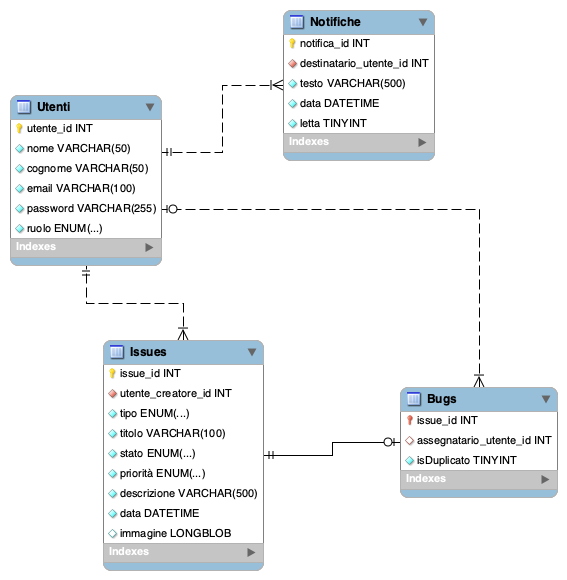
\includegraphics[width=\linewidth]{Chapters/schema ER.png}
\end{center}
\caption{Schema ER}
\label{fig:f1} 
\end{figure}

 La chiave gialla indica la chiave primaria, il rombo rosso una chiave esterna.
- Il rombo pieno indica una colonna obbligatoria (NOT NULL), quello vuoto una 
colonna facoltativa.
- La linea tratteggiata indica una relazione non identificante, la linea 
continua una relazione identificante, in cui la chiave esterna 
ùfa parte della chiave primaria (è il caso di Bugs).

\section{ Report di qualità del codice}
Lo strumento utilizzato per assicurare un ottimo livello di qualità 
del codice del back-end è stato SonarQube for IDE, plugin per IntelliJ. 
Sono stati risolti tutti i warning e i code smells durante lo sviluppo del progetto, 
e per il report finale è stato usato SonaeQube Cloud: qui di seguito il summary 
indicante due errori relativi alla sicurezza, ma che sono in realtà scelte deliberate.

\begin{figure}[!ht] 
\begin{center}
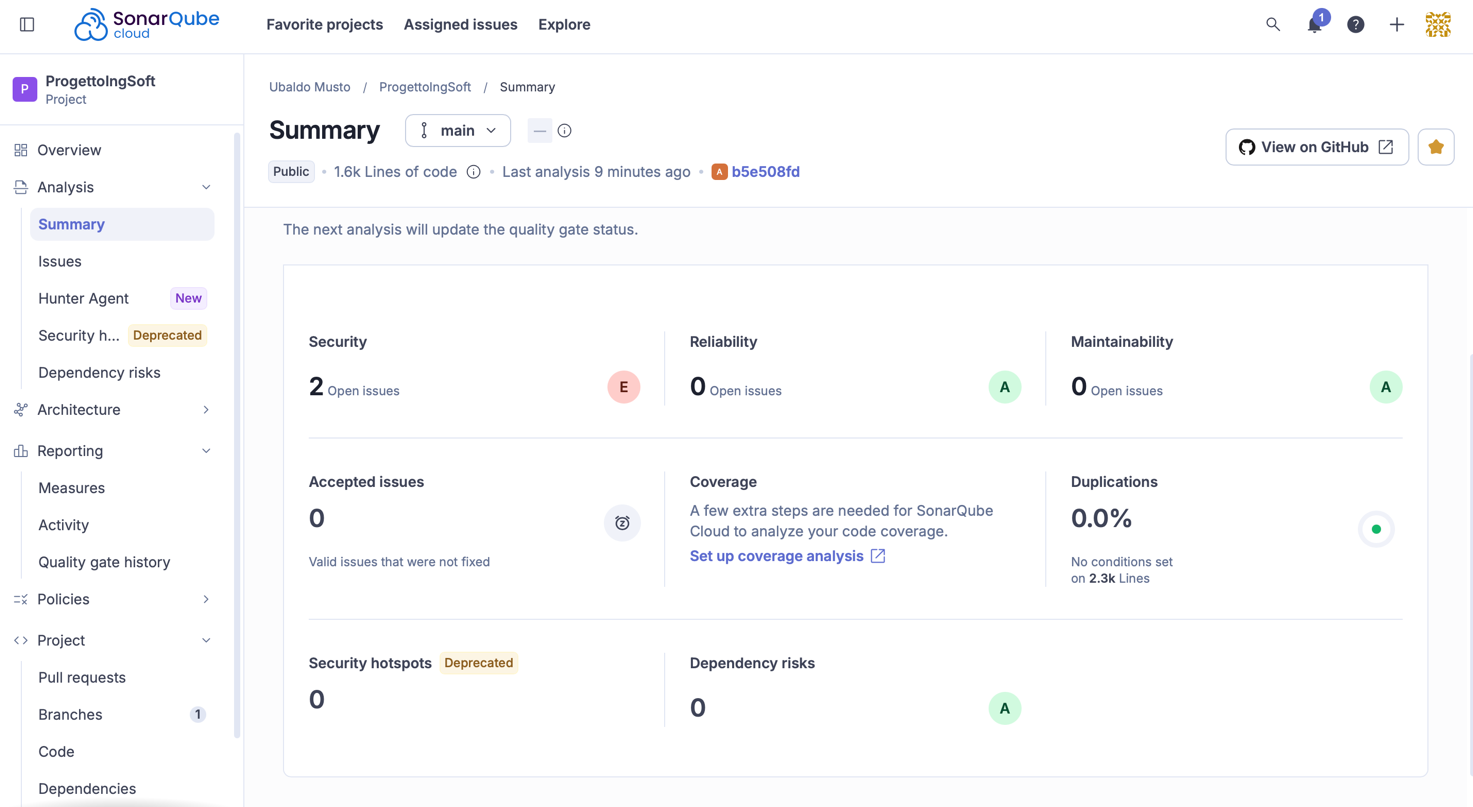
\includegraphics[width=\linewidth]{Chapters/report.png}
\end{center}
\caption{Report}
\label{fig:f1} 
\end{figure}

Data la natura del progetto si è optato di creare il primo utente admin direttamente 
dal codice, per ovviare a una moltitudine di problemi di testing e di demo su diverse
 macchine. Tale scelta però comporta la scrittura del nome utente ed ovviamente della 
 password (seppur sempre in formato hash) in maniera hardcoded, e ciò rappresenta una 
 falla di sicurezza.
Nel momento della messa in produzione del software una nuova migration Flyway risolve tutto.

\subsection{Make sure disabling Spring Security's CSRF protection is safe}
Questa problematica indica che la protezione CSRF (Cross-Site Request Forgery) di 
Spring Security è stata disattivata. Tale scelta è stata presa in quanto il CSRF è un 
attacco che sfrutta l'invio automatico dei cookie da parte del browser, ma il nostro
 client è un'applicazione JavaFX che gestisce da sé il cookie di sessione, quindi 
 l'attacco non è possibile e la protezione è stata disattivata.    
Se in futuro si aggiungesse un front-end web, la protezione andrebbe riattivata.   

\clearpage

\begin{figure}[!ht] 
\begin{center}
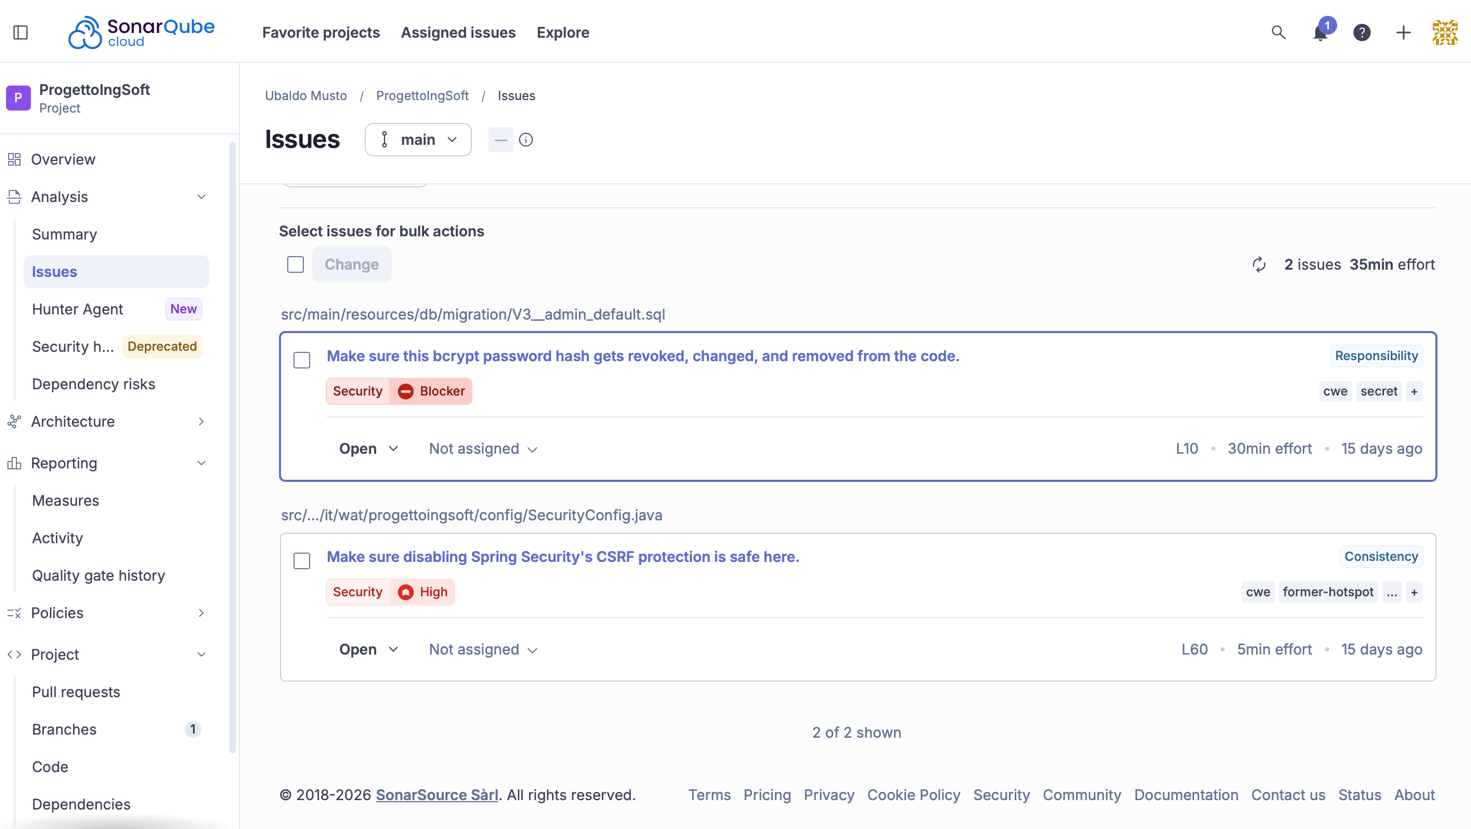
\includegraphics[width=\linewidth]{Chapters/report1.png}
\end{center}
\caption{Report}
\label{fig:f1} 
\end{figure}